%\documentclass[a4paper]{article}
\usepackage[utf8]{inputenc}
\usepackage[spanish, es-tabla, es-noshorthands]{babel}
\usepackage[table,xcdraw]{xcolor}
\usepackage[a4paper, footnotesep=1.25cm, headheight=1.25cm, top=2.54cm, left=2.54cm, bottom=2.54cm, right=2.54cm]{geometry}
%\geometry{showframe}

%\usepackage{wrapfig}			%Wrap figure in text
\usepackage[export]{adjustbox}	%Move images
\usepackage{changepage}			%Move tables

\usepackage{tikz}
\usepackage{amsmath}
\usepackage{amsfonts}
\usepackage{amssymb}
\usepackage{float}
\usepackage{graphicx}
\usepackage{caption}
\usepackage{subcaption}
\usepackage{multicol}
\usepackage{multirow}
\usepackage{wrapfig}
\setlength{\doublerulesep}{\arrayrulewidth}
\usepackage{booktabs}
\usepackage[numbib, nottoc, notlot, notlof]{tocbibind}

\usepackage{hyperref}
\hypersetup{
    colorlinks=true,
    linkcolor=blue,
    filecolor=magenta,      
    urlcolor=blue,
    citecolor=blue,    
}

%Change Font Size

% #1 = size, #2 = text
\newcommand{\setparagraphsize}[2]{{\fontsize{#1}{6}\selectfont#2 \par}}		%Cambia el size de todo el parrafo
\newcommand{\setlinesize}[2]{{\fontsize{#1}{6}\selectfont#2}}				%Cambia el font de una oración

\newcommand{\note}[1]{
	\begin{center}
		\huge{ \textcolor{red}{#1} }
	\end{center}
}

%FONTS (IMPORTANTE): Compilar en XeLaTex o LuaLaTeX
\usepackage{anyfontsize}	%Font size
\usepackage{fontspec}		%Font type

\usepackage{etoolbox}
\usepackage{todonotes}

\newcommand{\observacion}[2]{  \ifnumequal{1}{#1}{ { \todo[inline,backgroundcolor=red!25,bordercolor=red!100]{\textbf{Observación: #2}} } }{  }  }

\setcounter{topnumber}{2}
\setcounter{bottomnumber}{2}
\setcounter{totalnumber}{4}
\renewcommand{\topfraction}{0.85}
\renewcommand{\bottomfraction}{0.85}
\renewcommand{\textfraction}{0.15}
\renewcommand{\floatpagefraction}{0.8}
\renewcommand{\textfraction}{0.1}
\setlength{\floatsep}{5pt plus 2pt minus 2pt}
\setlength{\textfloatsep}{5pt plus 2pt minus 2pt}
\setlength{\intextsep}{5pt plus 2pt minus 2pt}

\newcommand{\quotes}[1]{``#1''}
\usepackage{array}
\newcolumntype{C}[1]{>{\centering\let\newline\\\arraybackslash\hspace{0pt}}m{#1}}
\usepackage[american]{circuitikz}
\usetikzlibrary{calc}
\usepackage{fancyhdr}
\usepackage{units} 

\graphicspath{{../Control de posición no lineal/}{../Control de fuerza no lineal/}{../Control híbrido no lineal/}{../Referencias/}{../Deducción de modelo/}{../Conclusiones/}}

\pagestyle{fancy}
\fancyhf{}
\lhead{22.99 - Automación Industrial}
\rhead{Lambertucci, Londero B., Maselli, Mechoulam}
\rfoot{Página \thepage}

%Items con bullets y no cuadrados
\renewcommand{\labelitemi}{\textbullet }

%%
%\begin{document}

\Subsection{Modelo Físico}
El doble péndulo invertido fue modelado como un manipulador Prismático-Rotacional-Rotacional. 
\begin{figure}[H]
	\centering
	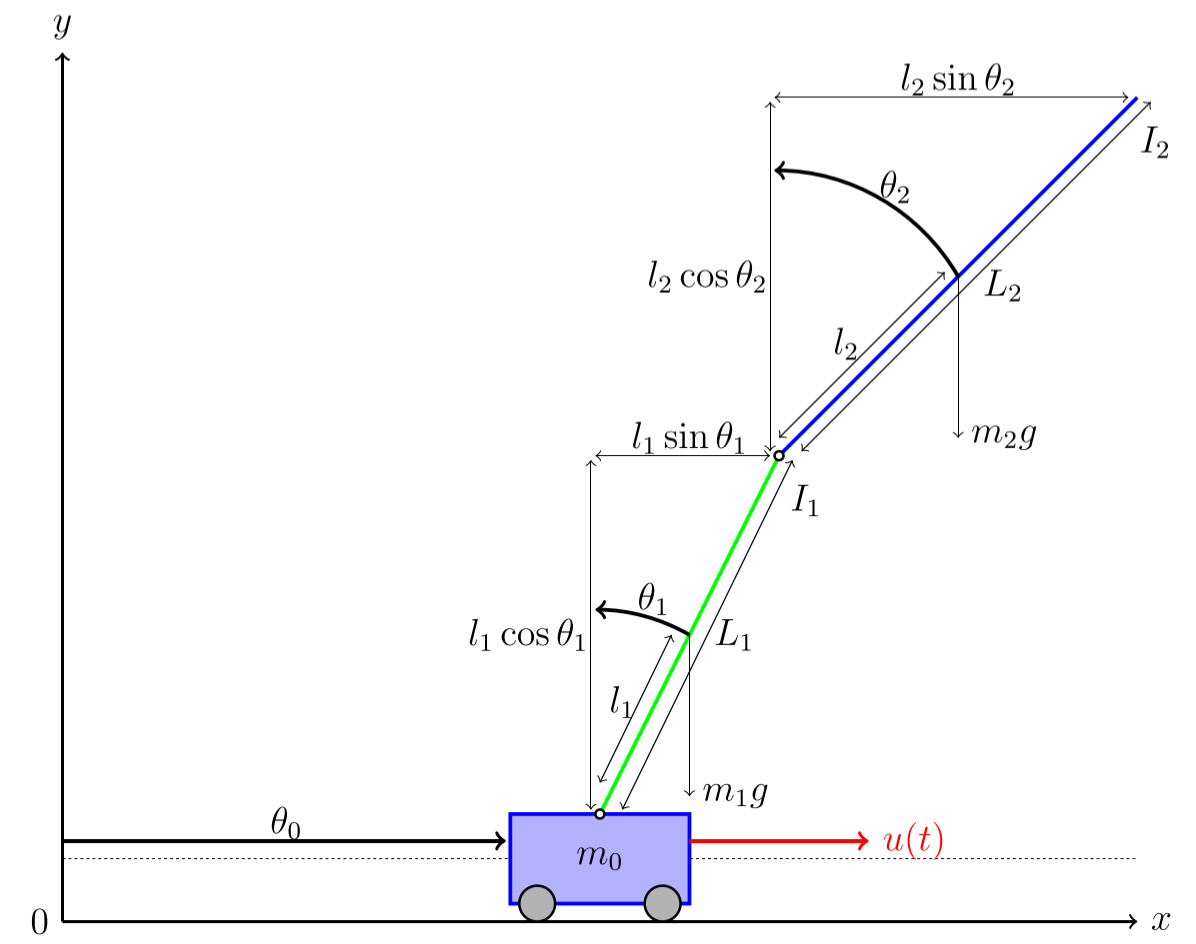
\includegraphics[width=\linewidth]{../Modelo Teorico/ImagenesModelo Teorico/sistema}
	\caption{Modelo teórico del doble péndulo invertido.}	
	\label{fig:pendteo}
\end{figure}
Luego utilizando la formulación de Euler-Lagrange.
\begin{equation}
  \frac{d}{dt}\frac{\partial L}{\partial \dot{\Theta}} - \frac{\partial L}{\partial \Theta}  = \tau
\end{equation} 
\begin{equation}
L\left( \Theta , \dot{\Theta} \right) = \sum_{i=0}^2
\left( \frac{1}{2} m_i v_{Ci}^Tv_{Ci} +\frac{1}{2} I_i \omega_{Ci}^T\omega_{Ci} + u_{refi} - m_i g d_{Ci}\right)
\end{equation} 
Se llega al sistema de segundo orden no lineal:
\begin{equation}
\tau = M\left( \Theta \right)\ddot{\Theta} + V\left( \Theta , \dot{\Theta} \right) + G\left( \Theta \right)
\end{equation}
Siendo las matrices:
\begin{equation}
 M\left( \Theta \right)\ddot{\Theta} = \begin{bmatrix}
m_0+m_1+m_2 & \left( m_1l_1 + m_2L_1 \right) \cos \theta_1 & m_2l_2 \cos \theta_2\\

\left( m_1l_1 + m_2L_1 \right) \cos \theta_1  &
m_1l_1^2+m_2L_1^2+I_1
& m_2L_1l_2\cos(\theta_1-\theta_2)\\


m_2l_2\cos\theta_2 & m_2L_1l_2\cos(\theta_1-\theta_2) & m_2l_2^2+I_2
\end{bmatrix}
\end{equation}
\begin{equation}
 V\left( \Theta , \dot{\Theta} \right) =
 \begin{bmatrix}
0 & -\left( m_1l_1 + m_2L_1 \right)\sin \theta_1 \dot{\theta_1} & -m_2l_2\sin \theta_2 \dot{\theta_2}\\
0 & 0 & m_2L_1l_2\sin(\theta_1-\theta_2)\dot{\theta_2}\\
0 & -m_2L_1l_2\sin(\theta_1-\theta_2)\dot{\theta_1} & 0
\end{bmatrix}
\end{equation}
\begin{equation}
 G\left( \Theta \right) = \begin{bmatrix}
0 \\
 -(m_1l_1+m_2L_1)g\sin\theta_1 \\
-m_2gl_2\sin\theta_2
\end{bmatrix}
\end{equation}
\begin{equation}
 H = \begin{bmatrix}
1 \\
 0 \\
0
\end{bmatrix}
\hspace{1cm}
\tau = H\cdot u(t)
\end{equation}
Si se asume los siguientes valores:
\begin{equation}
l1 = \frac{1}{2} L_1
\hspace{1cm}
l2 = \frac{1}{2} L_2 
\hspace{1cm}
I_1 = \frac{1}{12} m_1L_1^2
\hspace{1cm}
I_2 = \frac{1}{12} m_2L_2^2
\end{equation}
Se simplifica a :
\begin{equation}
 M\left( \Theta \right)\ddot{\Theta} = \begin{bmatrix}
m_0+m_1+m_2 & \left( \frac{1}{2}m_1L_1 + m_2 \right) L_1\cos \theta_1  \frac{1}{2}& m_2L_2 \cos \theta_2\\

\left(  \frac{1}{2}m_1 + m_2 \right) L_1 \cos \theta_1  &
\left( \frac{1}{3}m_1+m_2\right) L_1^2
&  \frac{1}{2}m_2L_1L_2\cos(\theta_1-\theta_2)\\


 \frac{1}{2}m_2L_2\cos\theta_2 &  \frac{1}{2}m_2L_1L_2\cos(\theta_1-\theta_2) &  \frac{1}{3}m_2L_2^2
\end{bmatrix}
\end{equation}
\begin{equation}
 V\left( \Theta , \dot{\Theta} \right) =
 \begin{bmatrix}
0 & -\left(  \frac{1}{2}m_1 + m_2\right)L_1\sin \theta_1 \dot{\theta_1} & - \frac{1}{2}m_2L_2\sin \theta_2 \dot{\theta_2}\\
0 & 0 &  \frac{1}{2}m_2L_1L_2\sin(\theta_1-\theta_2)\dot{\theta_2}\\
0 & - \frac{1}{2}m_2L_1L_2\sin(\theta_1-\theta_2)\dot{\theta_1} & 0
\end{bmatrix}
\end{equation}
\begin{equation}
 G\left( \Theta \right) = \begin{bmatrix}
0 \\
 - \frac{1}{2}(m_1+m_2)L_1g\sin\theta_1 \\
- \frac{1}{2}m_2gL_2\sin\theta_2
\end{bmatrix}
\end{equation}
\begin{equation}
 H = \begin{bmatrix}
1 \\
 0 \\
0
\end{bmatrix}
\hspace{1cm}
\tau = H\cdot u(t)
\end{equation}
Cabe mencionar que $M(\Theta)$ es una matriz simétrica no-singular, por lo que existe la inversa y también es simétrica.

\Subsection{Espacio de estados}
Luego de hacer la linealización del sistema :
\begin{equation}
 A = \begin{bmatrix}
0 &  0 & 0 & 1 &  0 & 0\\

0 &  0 & 0 & 0 &  1 & 0\\
0 &  0 & 0 & 0 &  0 & 1\\

0 &  -\frac{3g(2m_1^2 + 5m_1m_2 + 2m_2^2)}{2(4m_0m_1 + 3m_0m_2 + m_1m_2 + m_1^2} & 
\frac{3gm_1m_2}{2(4m_0m_1 + 3m_0m_2 + m_1m_2 + m_1^2}  & 0 &  0 & 0\\

0 &  \frac{3g(4m_1^2 + 9m_1m_2 + 4m_0m_1 + 2m_2^2 + 8m_0m_2)}{2L_1(4m_0m_1 + 3m_0m_2 + m_1m_2 + m_1^2)} & -\frac{9*g*(2m_0m_2 + m_1m_2)}{2L_1(4m_0m_1 + 3m_0m_2 + m_1m_2 + m_1^2)}
 & 0 &  0 & 0\\

0 &   -\frac{9g(2m_0m_1 + 4m_0m_2 + 2m_1m_2 + m_1^2)}{2L_2(4m_0m_1 + 3m_0m_2 + m_1m_2 + m_1^2)} & \frac{3g(4m_0m_1 + 12m_0m_2 + 4m_1m_2 + m_1^2)}{2L_2(4m_0m_1 + 3m_0m_2 + m_1m_2 + m_1^2)} & 0 &  0 & 0
\end{bmatrix}
\end{equation}
\begin{equation}
 B = \begin{bmatrix}
0 \\
0 \\
0 \\
\frac{4m_1 + 3m_2}{4m_0m_1 + 3m_0m_2 + m_1m_2 + m_1^2} \\
 -\frac{3(2m_1 + m_2)}{L_1(4m_0m_1 + 3m_0m_2 + m_1m_2 + m_1^2)} \\
\frac{2m_2}{L_2(4m_0m_1 + 3m_0m_2 + m_1m_2 + m_1^2)}
\end{bmatrix}
\end{equation}
Si se opta por los siguientes valores:
\begin{equation}
m_0 = 5 \ Kg
\hspace{0.5cm}
m_1 = 1 \ Kg
\hspace{0.5cm}
m_2 = 1 \ Kg
\hspace{0.5cm}
L_1 = 1 \ m
\hspace{0.5cm}
L_2 = 1.5 \ m
\hspace{0.5cm}
g= 9.8 \ \frac{m}{s^2}
\end{equation}
\
Se obtiene:

\begin{equation}
 A = \begin{bmatrix}
0 &  0 & 0 & 1 &  0 & 0\\
0 &  0 & 0 & 0 &  1 & 0\\
0 &  0 & 0 & 0 &  0 & 1\\
0 &  -3.5757 & 0.3973 & 0 &  0 & 0\\
0 &  29.7973 & -13.1108 & 0 &  0 & 0\\
0 &  -26.2216 & 22.5135 & 0 &  0 & 0
\end{bmatrix}
\end{equation}
\begin{equation}
 B = \begin{bmatrix}
0 \\
0 \\
0 \\
0.1892 \\
-0.2432 \\
0.036 
\end{bmatrix}
\end{equation}

\Subsection{Controlabilidad y Observabilidad}
\label{sec:ctrbyobsv}

Se define al set de estados alcanzables $\mathcal{R}_t$ en un tiempo $t$ como aquellos estados en los que el sistema se puede encontrar. Por otro lado, se define al subespacio controlable $\mathcal{C}_{AB}$ como aquellos estados a los que se puede forzar el sistema mediante una entrada $u(t)$ apropiada. Se puede probar que para $t > 0$ el set de estados alcanzables $\mathcal{R}_t$ es igual que el subespacio controlable $\mathcal{C}_{AB}$. \cite{ref:dullerud}

Se dice que el par $(A, B)$ es controlable, y por ende un sistema definido con esas matrices es controlable si la matriz de controlabilidad

\begin{equation}
[B \ AB \ \cdots \ A^{n-1}B]
\end{equation}

es de rango completo.

Para el caso del péndulo doble, se tiene que

\begin{equation}
[B \ AB \ \cdots \ A^{n-1}B] = 	\begin{bmatrix}
0       &  0.1892  & 0        & 0.8839  &  0         & 30.4554\\
0       &  -0.2432 & 0        & -7.7189 &  0         & -324.2311\\
0       &  0.0360  & 0        & 7.1876  &  0         & 364.2140\\
0.1892  &  0       & 0.8839   & 0       &  30.4554   & 0\\
-0.2432 &  0       & -7.7189  & 0       &  -324.2311 & 0\\
0.0360  &  0       & 7.1876   & 0       &  364.2140  & 0
\end{bmatrix}
\end{equation}

donde se puede observar que la matriz es de rango completo, por lo que el sistema es controlable.

%Otro método más sofisticado para probar la controlabilidad de un sistema es el Test PBH, el cual se basa 

Otros dos aspectos importantes del sistema son la detectabilidad y la observabilidad, dado que en la vida real muchas veces no es posible medir todas las variables del sistema. 

El estudio de la observabilidad del sistema se basa en comprobar la posibilidad de estimar las variables de estado a partir de la salida. Por otro lado, un estudio más débil pero de igual importancia teórica es la detectabilidad. Un sistema es detectable si todos sus estados no observables son estables. Se puede probar que si el par $(C^*,A^*)$ es controlable, entonces el par $(A,C)$ es observable. 

En el caso del problema estudiado, se tiene que, midiendo la posición del carrito y las dos posiciones angulares, es decir

\begin{equation}
C = 	\begin{bmatrix}
1 & 0 & 0 & 0 & 0 & 0\\
0 & 1 & 0 & 0 & 0 & 0\\
0 & 0 & 1 & 0 & 0 & 0
\end{bmatrix}
\end{equation}

luego

\begin{equation}
[C^* \ A^*C^* \ \cdots \ A^{*n-1}C^*]
\end{equation}

es de rango completo, por lo que el sistema será observable midiendo las variables de estado definidas por la matriz C.
\Subsubsection{Estudio con diagramas de Mason}
En la modelización de la planta como se verá en la seccion (\ref{sec:simulacionessimscape}) se debate entre el sistema con y sin fricción.
Por lo que a continuación se define la observabilidad y controlabilidad de ambos sistemas. Por lo que se realizaron los diagramas de Mason para cada sistema.
Asumiendo un espacio en variables de la siguiente forma:
\begin{equation}
 A = \begin{bmatrix}
0 &  0 & 0 & 1 &  0 & 0\\
0 &  0 & 0 & 0 &  1 & 0\\
0 &  0 & 0 & 0 &  0 & 1\\
0 &  a & b & c &  d & e\\
0 &  f & g & h &  i & j\\
0 &  k & l & m &  n & o
\end{bmatrix}
\end{equation}
\begin{equation}
 B = \begin{bmatrix}
0 \\
0 \\
0 \\
b_1 \\
b_2 \\
b_3 
\end{bmatrix}
\end{equation}
\begin{equation}
C = 	\begin{bmatrix}
c_1 & 0 & 0 & 0 & 0 & 0\\
0 & c_2 & 0 & 0 & 0 & 0\\
0 & 0 & c_3 & 0 & 0 & 0
\end{bmatrix}
\end{equation}
\Subsubsubsection{Sistema con fricción y mediciones de $\theta_1$, $\theta_2$ y $x_0$}
A continuación se ve el diagrama de Mason para el sistema mencionado.
\begin{figure}[H]
	\centering
	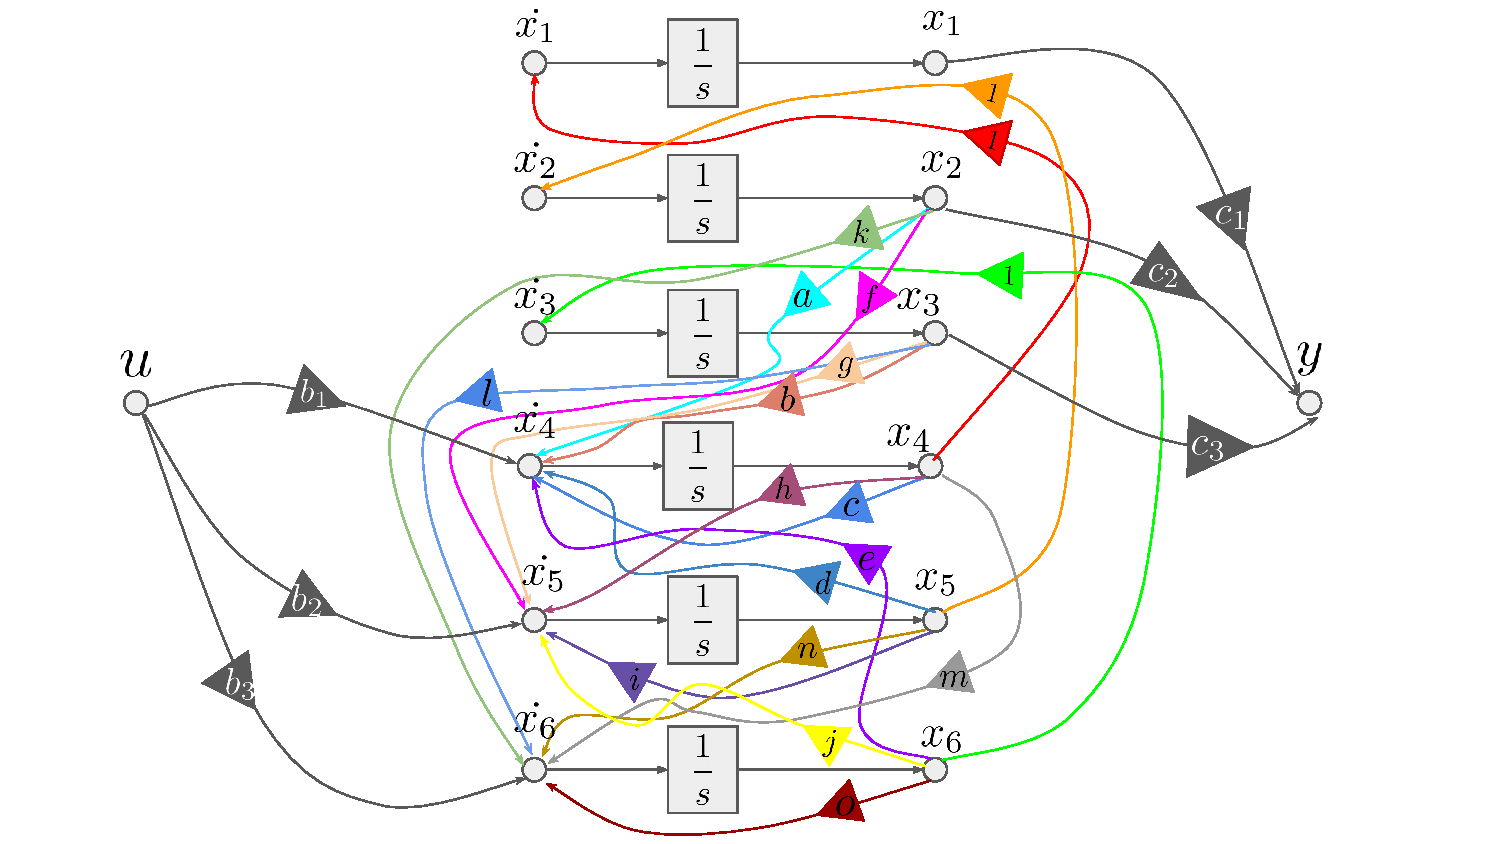
\includegraphics[width=1\linewidth,page = 1]{../Modelo Teorico/ImagenesModelo Teorico/Mason.pdf}
	\caption{Diagrama de Mason del sistema con fricción y mediciones de $\theta_1$, $\theta_2$ y $x_0$.}	
	\label{fig:masonsisfyxomf}
\end{figure}

En el caso de la controlabilidad se hará un solo estudio debido a que es el mismo para los 3 casos que observaremos. Se observa que se puede llegar desde la acción de control a todas las variables de estado con un recorrido corto.
\begin{figure}[H]
	\centering
	\includegraphics[width=1\linewidth,page = 2]{../Modelo Teorico/ImagenesModelo Teorico/Mason.pdf}
	\caption{Diagrama de Mason marcando la controlabilidad.}	
	\label{fig:masonsisfyxofmC}
\end{figure}
Luego veremos la observabilidad, que en el caso del sistema con fricción y midiendo la posición y ángulos, se nota que el nivel de anidamiento de las variables de estado es de un solo nivel, teniendo que para medir las variables $x_6$, $x_5$ y $x_4$, basta con derivar las salidas. 
\begin{figure}[H]
	\centering
	\includegraphics[width=1\linewidth,page = 3]{../Modelo Teorico/ImagenesModelo Teorico/Mason.pdf}
	\caption{Diagrama de Mason marcando la observabilidad.}	
	\label{fig:masonsisfyxofmO}
\end{figure}
Por lo que el sistema es sumamente observable.
\Subsubsubsection{Sistema con fricción y mediciones de $x_0$}
Aqui se muestra el diagrama de mason del sistema con fricción y mediciones únicamente de $x_0$. Este sistema tiene la particularidad de que al tener una única salida por $x_1$ llegar a todas las variables de estado se torna mas dificil.
\begin{figure}[H]
	\centering
	\includegraphics[width=1\linewidth,page = 4]{../Modelo Teorico/ImagenesModelo Teorico/Mason.pdf}
	\caption{Diagrama de Mason del sistema con fricción y mediciones de $x_0$.}	
	\label{fig:masonsisfyxom}
\end{figure}
Aqui veremos el camino que debe realizar cada variable de estado para llegar a la salida, o visto de otra manera el camino inverso que debe hacer el observador para estimar dichas variables.
\begin{figure}[H]
	\centering
	\includegraphics[width=1.2\linewidth,page = 5]{../Modelo Teorico/ImagenesModelo Teorico/Mason.pdf}
	\caption{Diagrama de Mason marcando observabilidad.}	
	\label{fig:masonsisfyxomO}
\end{figure}
Se observa que En este caso el camino hacia la salida es mucho menos directo, y todas las variables de estado pasan por la variable $x_4$ por lo que el anidamiento es superior al caso anterior y estimar las variables se torna mas dificil, teniendo en cuenta que ahora estan multiplicadas por las ganancias $a,b,c,$ etc.
Si bien en el sentido estricto de la palabra el sistema es completamente observable al igual que el anterior, en una aplicación real, teniendo en cuenta las diversas fuentes de ruido, este sistema resulta significativamente mas difícil de observar.
\Subsubsubsection{Sistema sin fricción y mediciones de $x_0$}
Finalmente observaremos el caso del sistema ideal sin fricción, midiendo únicamente la posición. El diagrama de Mason correspondiente es el siguiente:
\begin{figure}[H]
	\centering
	\includegraphics[width=1\linewidth,page = 6]{../Modelo Teorico/ImagenesModelo Teorico/Mason.pdf}
	\caption{Diagrama de Mason del sistema sin fricción y mediciones de $x_0$.}	
	\label{fig:masonsisyxom}
\end{figure}
En este caso se observa el mayor nivel de anidamiento de los 3 casos, resultando en el sistema que si se intentase replicar en la realidad menos probabilidad de éxito tendría. Si bien en el caso ideal funcionaría no es así en la realidad.
\begin{figure}[H]
	\centering
	\includegraphics[width=1\linewidth,page = 7]{../Modelo Teorico/ImagenesModelo Teorico/Mason.pdf}
	\caption{Diagrama de Mason marcando observabilidad.}	
	\label{fig:masonsisyxomO}
\end{figure}

%\end{document}
